\section{Institutional Background}\label{sec:inst}
%\pagenumbering{arabic}
\setstretch{1.5}

The promulgation of the \citeyear{constituicao} Brazilian Federal Constitution (CF/1998) promoted profound changes in the provision of health care in Brazil as it established universal and egalitarian access to health care as a constitutional right. Under this context, the Unified Health System (\emph{Sistema Único de Saúde} -- SUS) was created to provide free and universal health care to all citizens. The CF/1988 also established that the provision of health care would be financed by the Social Security System budget, together with social assistance and the public pension system, with resources coming from the federal, state and municipal budgets, and specific tax instruments. The implementation of new social rights, in a period of hyperinflation and macroeconomic restrictions, led to several budget disputes and crisis in the financing of health care \citep{Piola2013}. In order to secure resources for the SUS, the \nth{29} Constitutional Amendment (\emph{Emenda Constitutional 29} -- EC/29) was enacted in September of 2000.

In August of 1999 the President of the Brazilian Lower House determined the attachment of two Constitutional Amendment Proposals (\emph{Proposta de Emenda Constitucional} - PEC) -- 169 of 1992 and 82 of 1995 -- into a new proposal. While the PEC/169 intended to secure 30\% of the federal Social Security budget to the provision of public health care and 10\% of state and municipalities tax income, the PEC/82 intended to secure all resources from taxes over profits and revenues, that were originally financing the whole Social Security budget, to the provision of health care. The new proposal was approved by the Lower House in November of 1999 and sent to the Upper House, where it was approved in September of 2000 as the EC/29.

The EC/29 established the minimum share of resources that the federal, state and municipal governments need to spend on the provision of public health services. According to Art. \nth{7} of EC/29, from 2000 to 2004, the federal government should spend in the year of 2000 the amount spent in 1999 increased in 5\% and from 2001 to 2004 correct this value by the GDP growth; the state governments should spend 12\% of its tax income net of transfers to municipal governments; and municipalities should spend 15\% of its tax income (own resource spending). The states and municipalities spending less than the amount established when the EC/29 was enacted would have to gradually increase its expenditure, decreasing the distance to the target by at least one fifth a year and spending at least 7\% of its tax income \footnote{The EC/29 established the shares of resources that governments needed to spend only until 2004. A Complementary Law would have to be approved to regulate the EC/29 from 2005 on. In the a absence of a Complementary Law the share of resources defined by the Art. \nth{7} would apply. The Complementary Law was only approved in 2012, but it made no changes to the Art. \nth{7}}. 

\begin{figure}[h!]
    \begin{center}
    \caption{\footnotesize Spending Density Plots}\label{fig:density}
    \begin{subfigure}{0.48\textwidth}
        \caption{\scriptsize Health Spending (\% of own resources)}\label{fig:density_a}
        \centering
        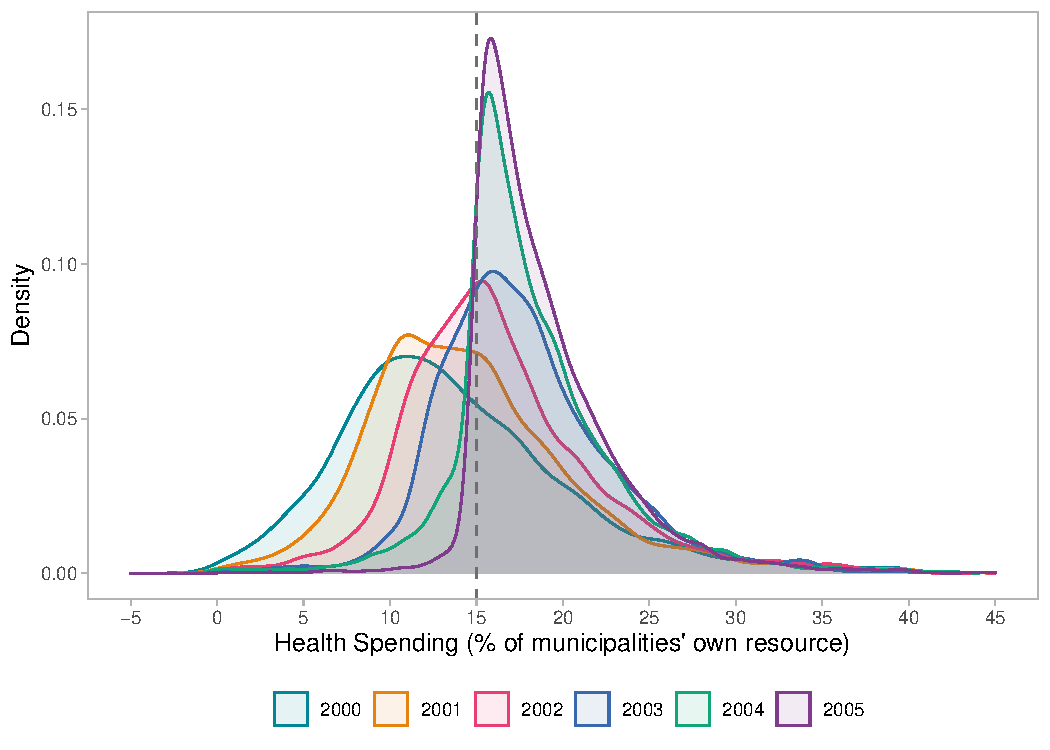
\includegraphics[width=\textwidth]{plots/hist_ec29.pdf}
    \end{subfigure}
        \begin{subfigure}{0.48\textwidth}
        \caption{\scriptsize Health Spending per capita (2010 R\$)}\label{fig:density_b}
        \centering
        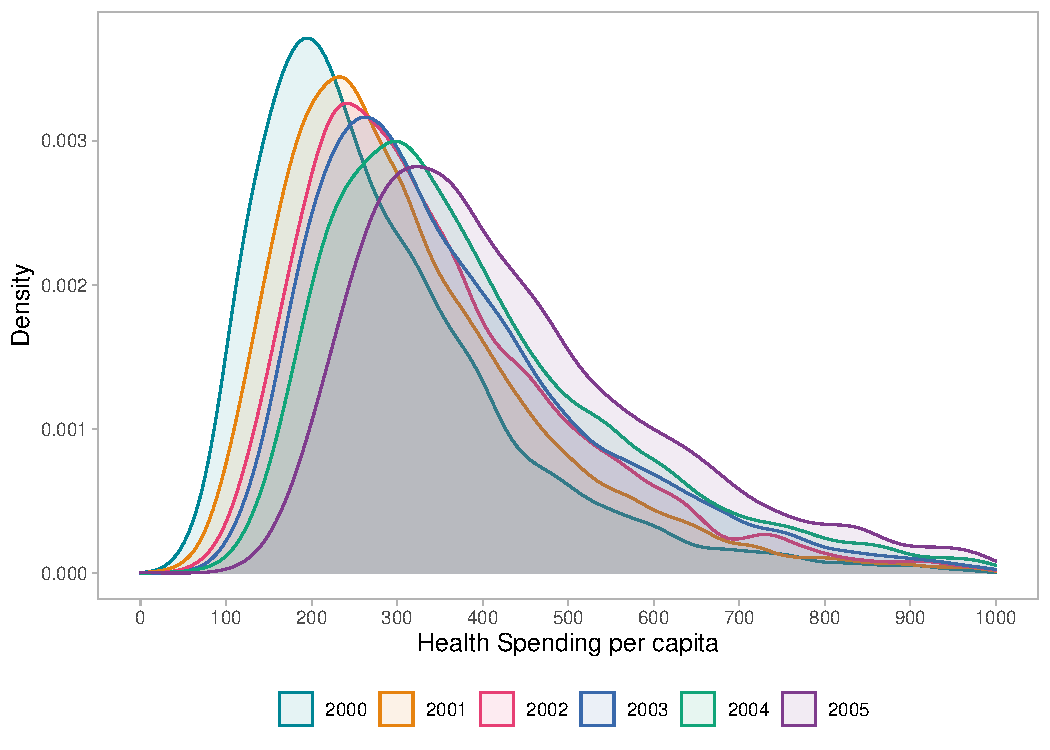
\includegraphics[width=\textwidth]{plots/hist_pc.pdf}
    \end{subfigure}
    \end{center}\vspace{+1pt}
    
    \floatfoot{    \scriptsize{Notes: Density plots calculated using SIOPS data (see Section \ref{sec:data} for more details). Dotted line in Figure \ref{fig:density_a} marks the EC/29 target (see Section \ref{sec:inst} for more details).}}

\end{figure}

\subsection{Municipalities Health Expenditure after the EC/29}

Figure \ref{fig:density_a} shows the distribution of municipalities according to their share of own resources spent in public health. While in 2000, our baseline year, most of the municipalities spent less than 15\%, in 2005 the great majority of municipalities were complying with the target stipulated by the EC/29. Figure \ref{fig:density_b} presents the distribution of municipalities according to their health spending per capita (in 2010 R\$). One could suggest two facts about this figure. First, there was a significant increase in the average health spending per capita and second, there was also some increase in the inequality of health spending per capita across municipalities.\footnote{\cite{Piola2013} highlights that the EC/29 provided a broad definition of health care that led some states and municipalities to include in this account expenditures that should not be considered part of expenditures related to the provision of public health services by the SUS.}


Figure \ref{fig:2} present trends in health spending at the municipality level converted into indices set at 100 in 2000, for the bottom and top quartile of the distribution of the share of own resources spent in health care. Figure \ref{fig:2a} shows that the municipalities in the bottom of the distribution presented much higher increase in health spending relative to the municipalities on the top of the distribution. Moreover, as shown in Figure \ref{fig:2b} and \ref{fig:2c}, expenditure coming from own resources explains almost all the difference in the health spending increase between the bottom and top quartile. Figure \ref{fig:3} plots trends for health spending per capita by source. Own resources has always been the main source of public health spending for municipalities, but the trends suggest that it gain even more importance after the EC/29 (Figure \ref{fig:3a}). In the baseline year of 2000, health spending per capita in the bottom quartile was half of the top quartile. Figures \ref{fig:3b} and \ref{fig:3b} suggest that all these difference comes from differential own resource spending. \cite{Piola2013} shows that states and municipalities own resource spending was responsible for about two thirds of the increase in health spending between 2000 and 2011.

\begin{figure}[h!]
    \begin{center}
    \caption{\footnotesize Health Spending Trends}\label{fig:2}
    \begin{subfigure}{.9\textwidth}
        \caption{\scriptsize Total Health Spending (2000 = 100)}\label{fig:2a}
        \centering
        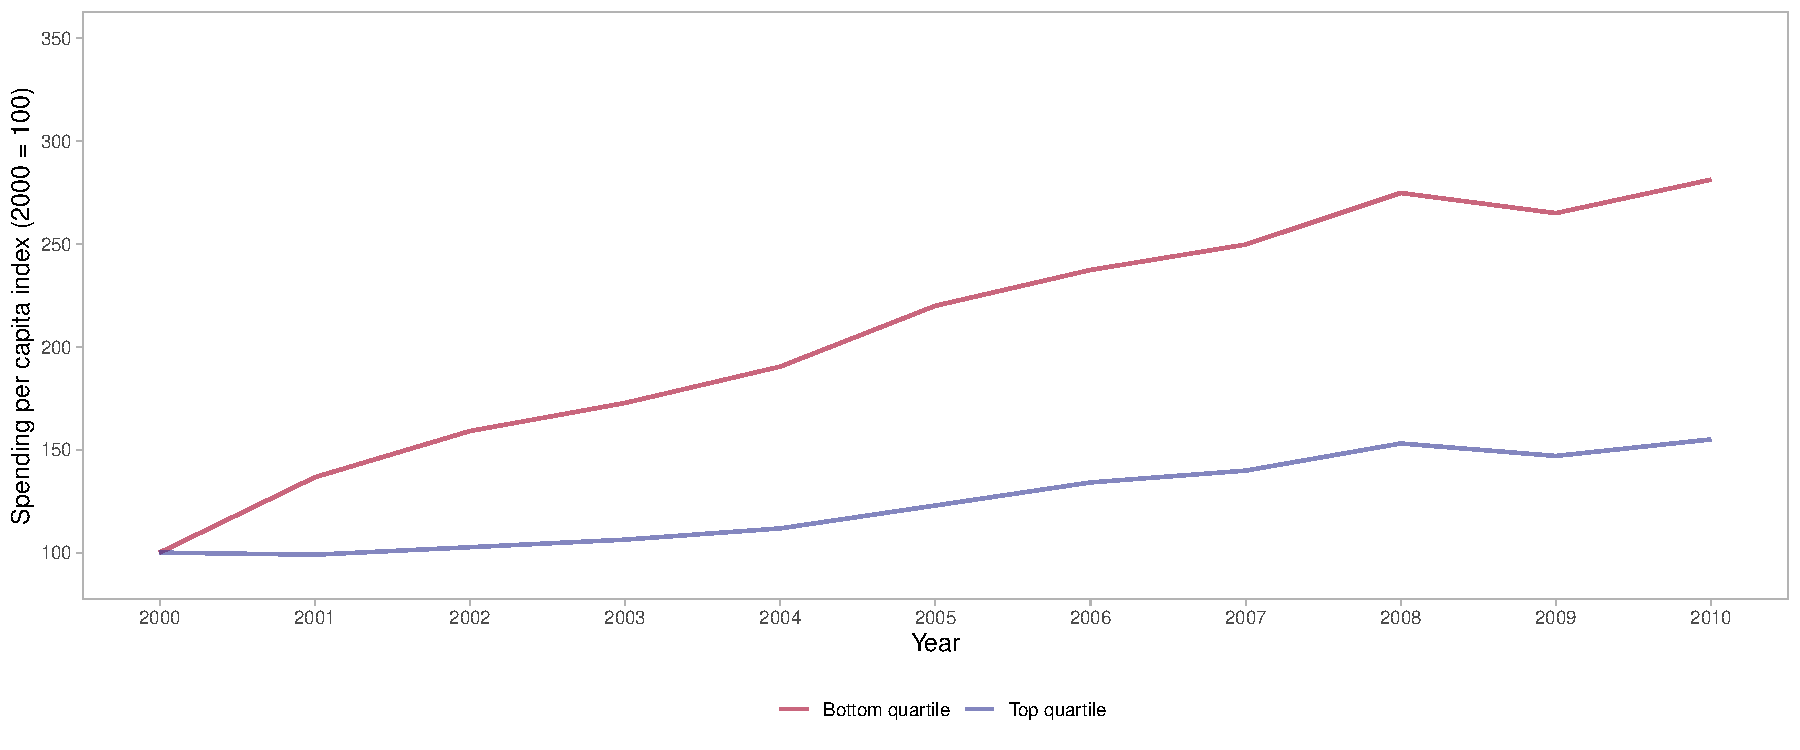
\includegraphics[width=\textwidth]{plots/plot_total.pdf}
    \end{subfigure}
        \begin{subfigure}{0.45\textwidth}
        \caption{\scriptsize Health Spending from Own Resources (2000 = 100)}\label{fig:2b}
        \centering
        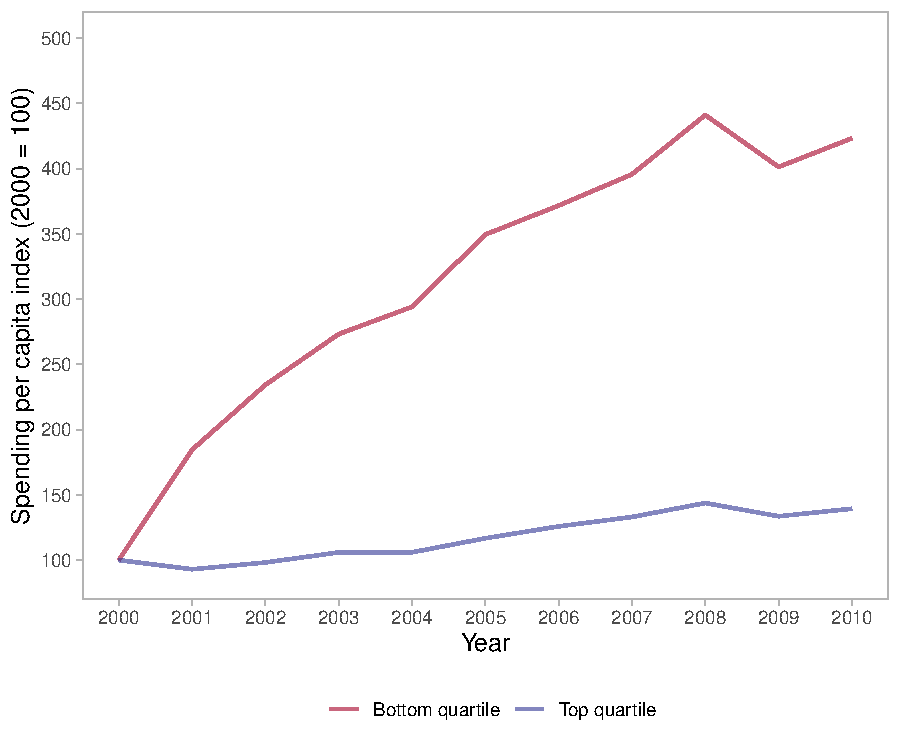
\includegraphics[width=\textwidth]{plots/plot_own.pdf}
    \end{subfigure}
        \begin{subfigure}{0.45\textwidth}
        \caption{\scriptsize Health Spending from Transfers (2000 = 100)}\label{fig:2c}
        \centering
        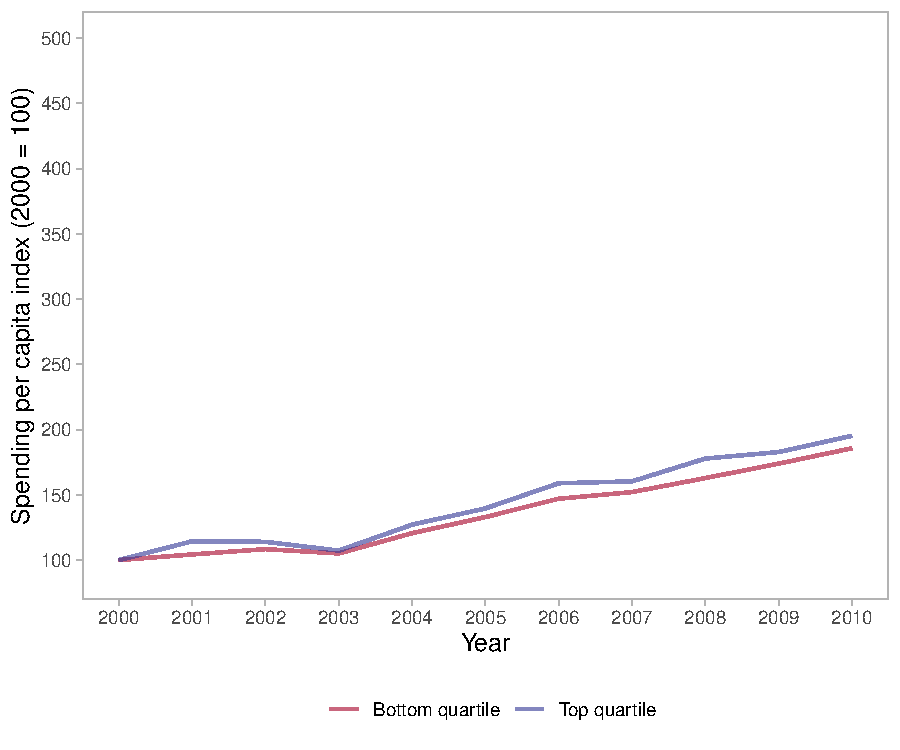
\includegraphics[width=\textwidth]{plots/plot_transf.pdf}
    \end{subfigure}
    \end{center}\vspace{+1pt}
\end{figure}
\begin{figure}[h!]
    \begin{center}
    \caption{\footnotesize Health Spending Trends}\label{fig:3}
    \begin{subfigure}{.9\textwidth}
        \caption{\scriptsize Health Spending by Source (R\$2010) - Full Sample}\label{fig:3a}
        \centering
        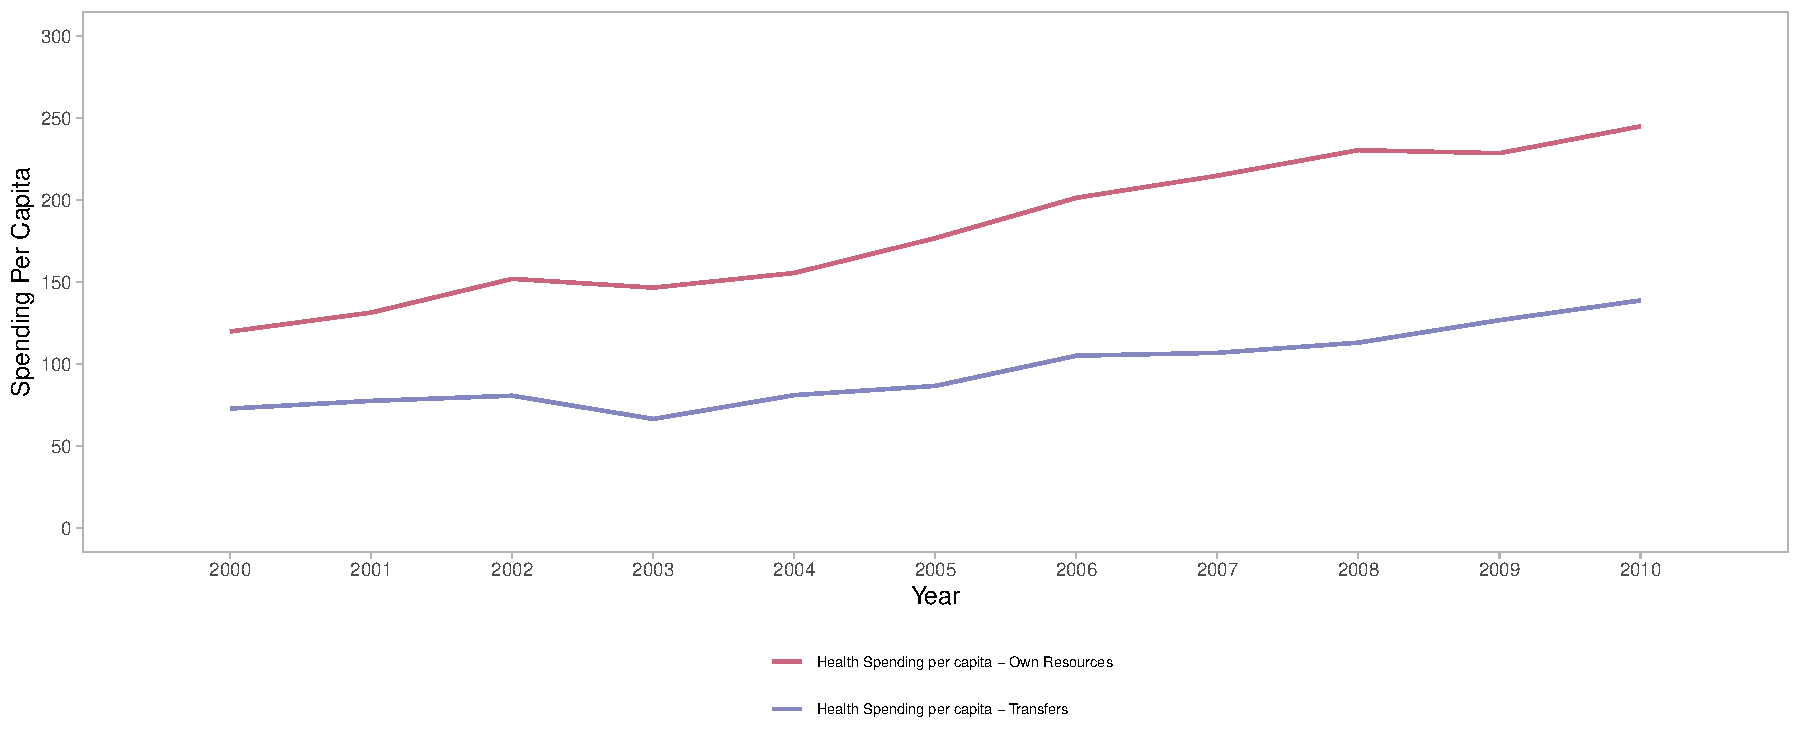
\includegraphics[width=\textwidth]{plots/plot_siops_level_source.pdf}
    \end{subfigure}
        \begin{subfigure}{0.45\textwidth}
        \caption{\scriptsize Health Spending by Source (R\$2010) - Bottom Quartile}\label{fig:3b}
        \centering
        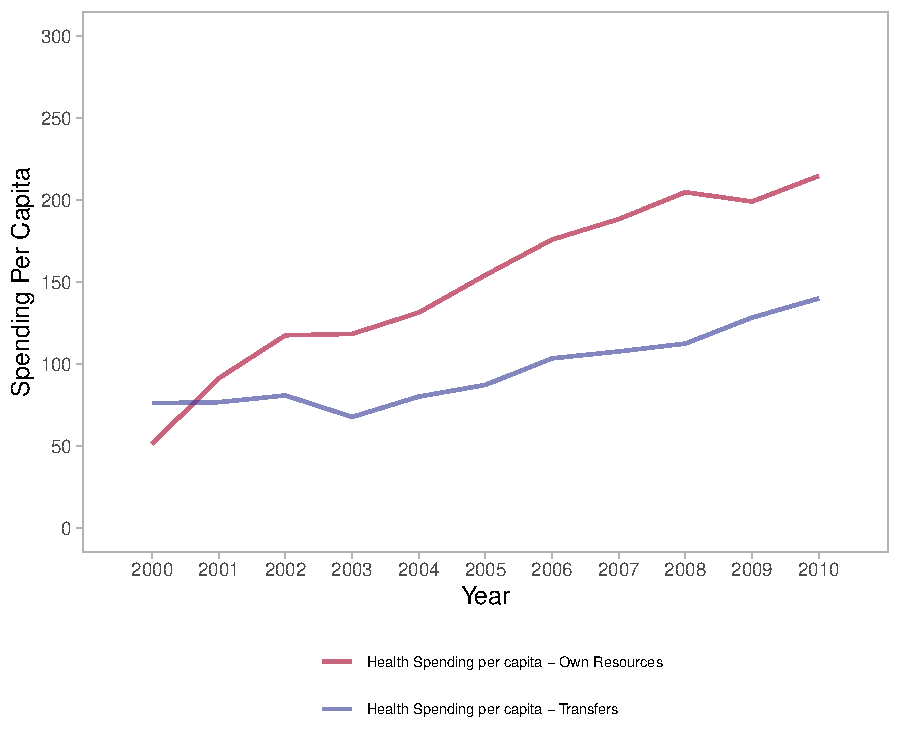
\includegraphics[width=\textwidth]{plots/plot_siops_level_source_bottom.pdf}
    \end{subfigure}
        \begin{subfigure}{0.45\textwidth}
        \caption{\scriptsize Health Spending by Source (R\$2010) - Top Quartile)}\label{fig:3c}
        \centering
        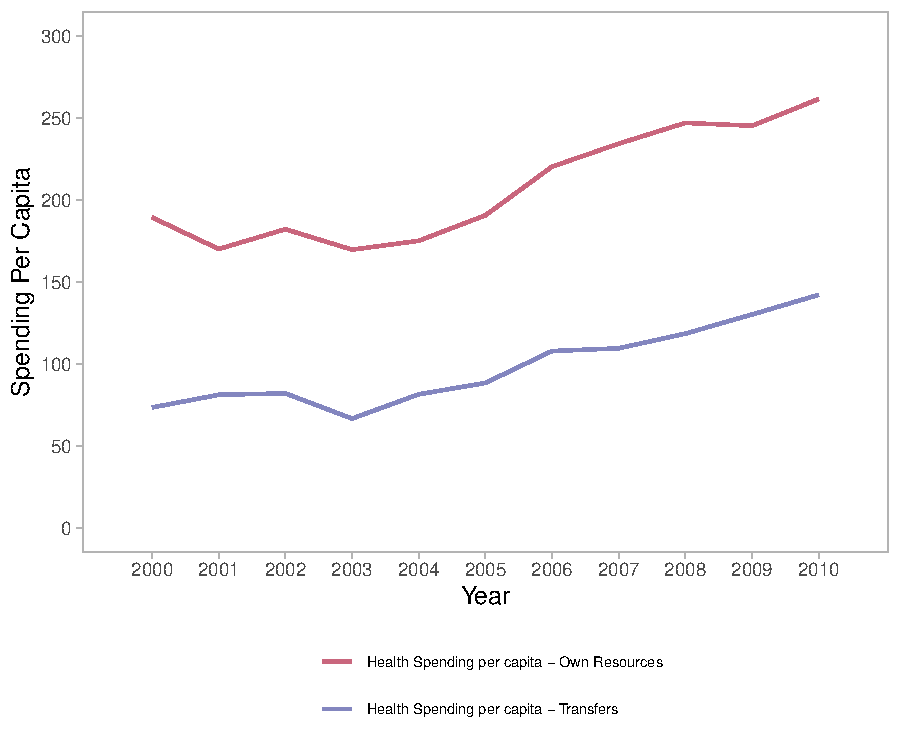
\includegraphics[width=\textwidth]{plots/plot_siops_level_source_top.pdf}
    \end{subfigure}
    \end{center}\vspace{+1pt}
    \scriptsize{Notes: Trends calculated using SIOPS spending data (see Section \ref{sec:data} for more details).}
\end{figure}


Moreover, municipalities' baseline level of own resource spending in health presents ample variation and is somewhat predictive of the change in total health spending per capita, which will be crucial to our identification strategy. Figure \ref{fig:4} plots, for all municipalities, the distance in percentage points to the EC/29 own resource spending target\footnote{We choose to work with the distance the target instead of the share of own resource expenditure in health in order to have easier to interpret estimates, as this measures presents a positive correlation with health spending} versus the change in total health spending per capita between 2000 and 2005. Consistently with the evidence presented in figure \ref{fig:2} and \ref{fig:3}, increases in health spending were larger in places with initially low levels of own resource spending, with a moderate to strong correlation of $0.45$.


\begin{figure}[h!]
\begin{center}
    \caption{Changes in Health Spending per capita (2000-2005)}
    \scalebox{0.7}{
    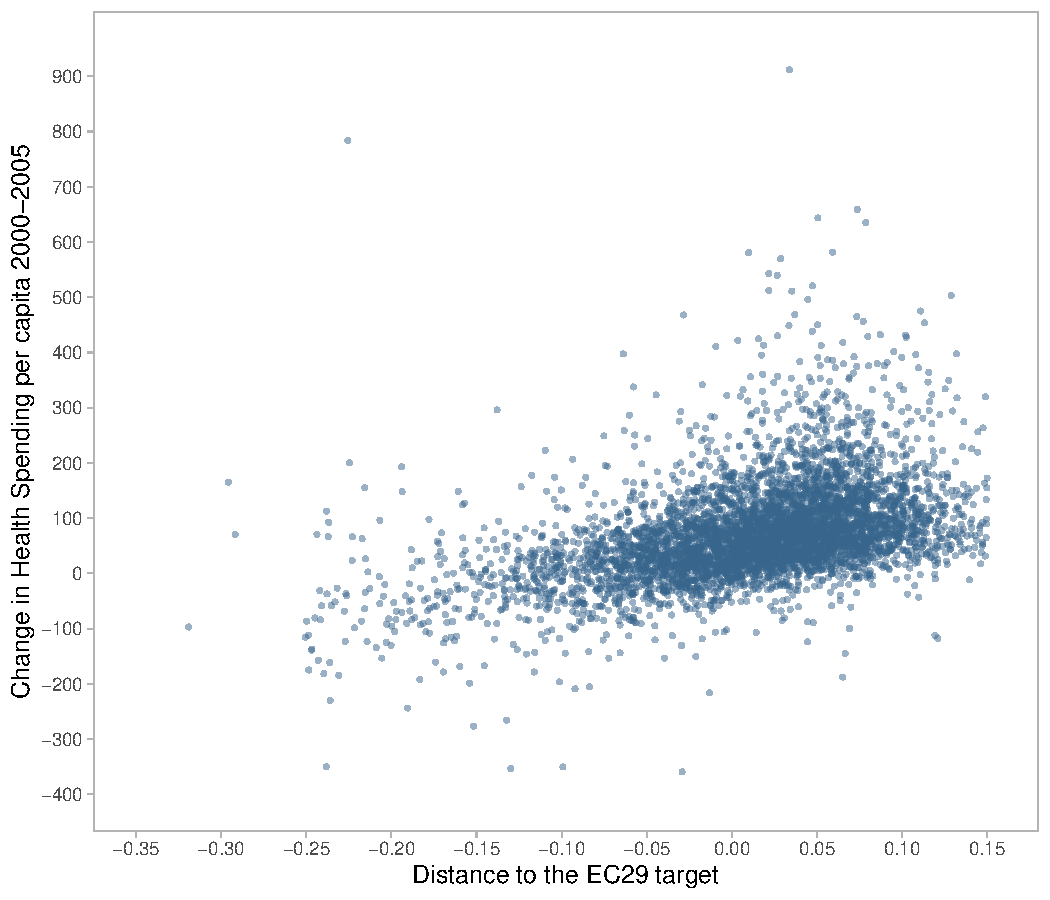
\includegraphics{plots/scatter_dist_ec29_baseline_change05.pdf}
    \label{fig:4}
    }
\end{center}
\end{figure}


In general, the descriptive evidence suggests that the EC/29 was responsible for bringing more resources to the provision of public health services and increasing the direct participation of states and municipalities in the financing of health care.
